% !TEX root = presentation.tex
%LTeX: language=de-CH

% \begin{frame}
%   \frametitle{Forecast: 01-May-2025 at 00:00, Level 850 hPa}
%   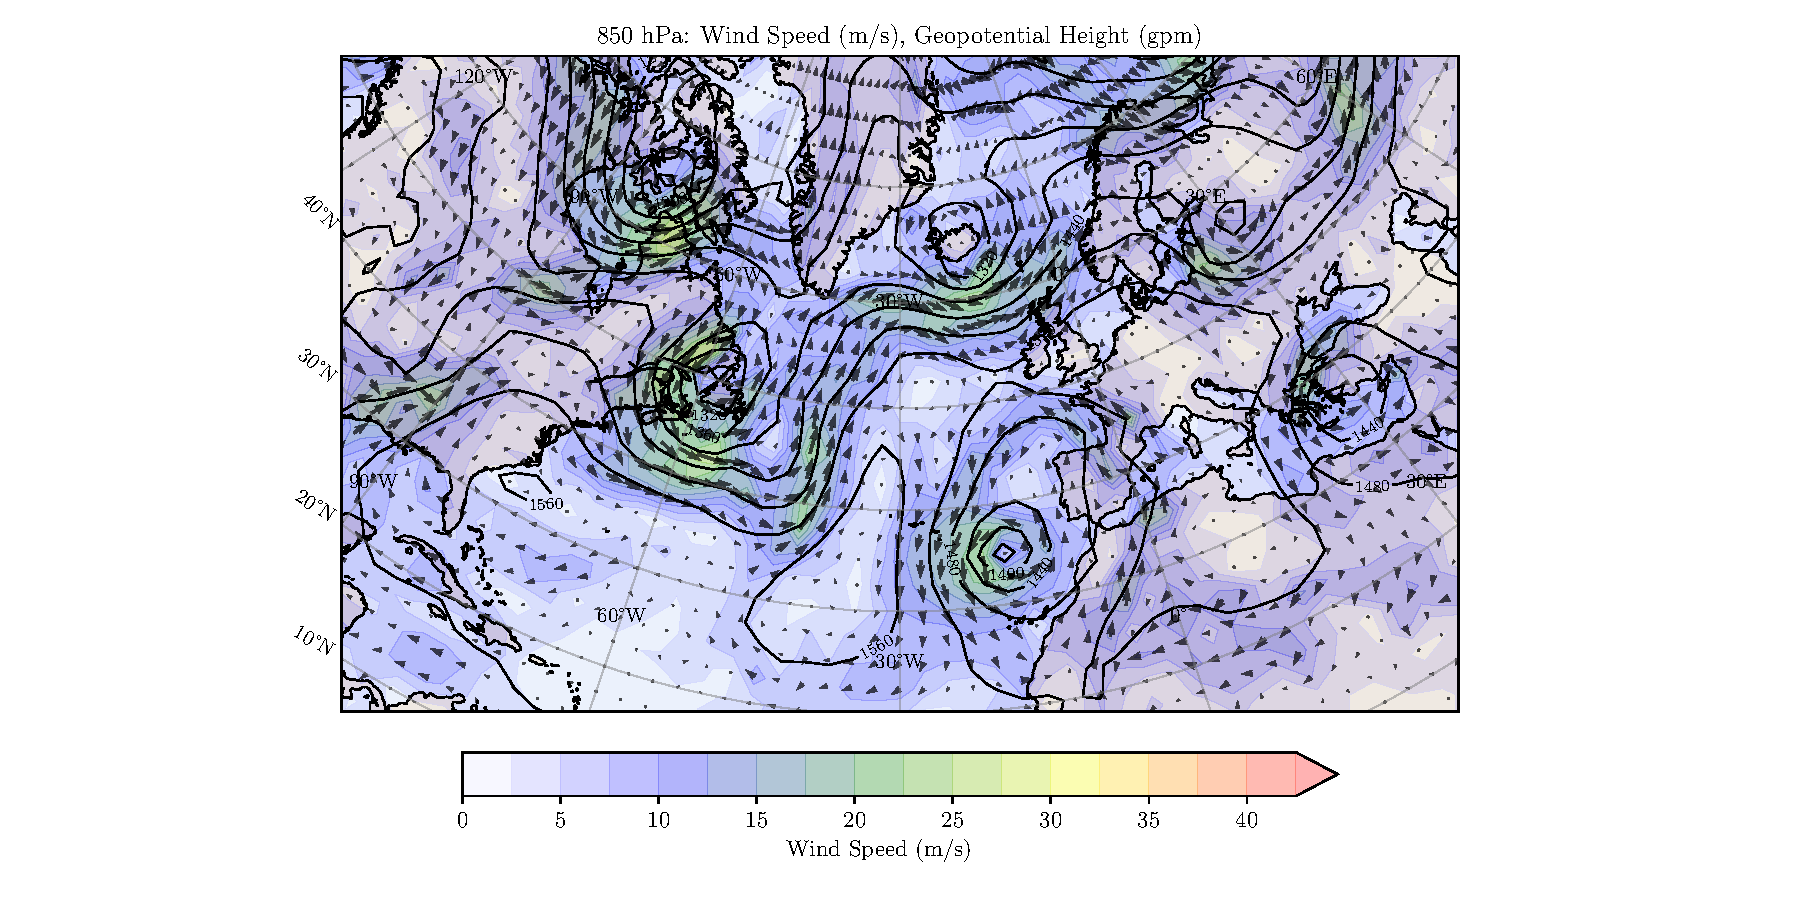
\includegraphics[width=\textwidth]{../images/weather/data_2025_5_1_00:00_850.pdf}
% \end{frame}
% \begin{frame}
%   \frametitle{Forecast: 01-May-2025 at 00:00, Level 500 hPa}
%   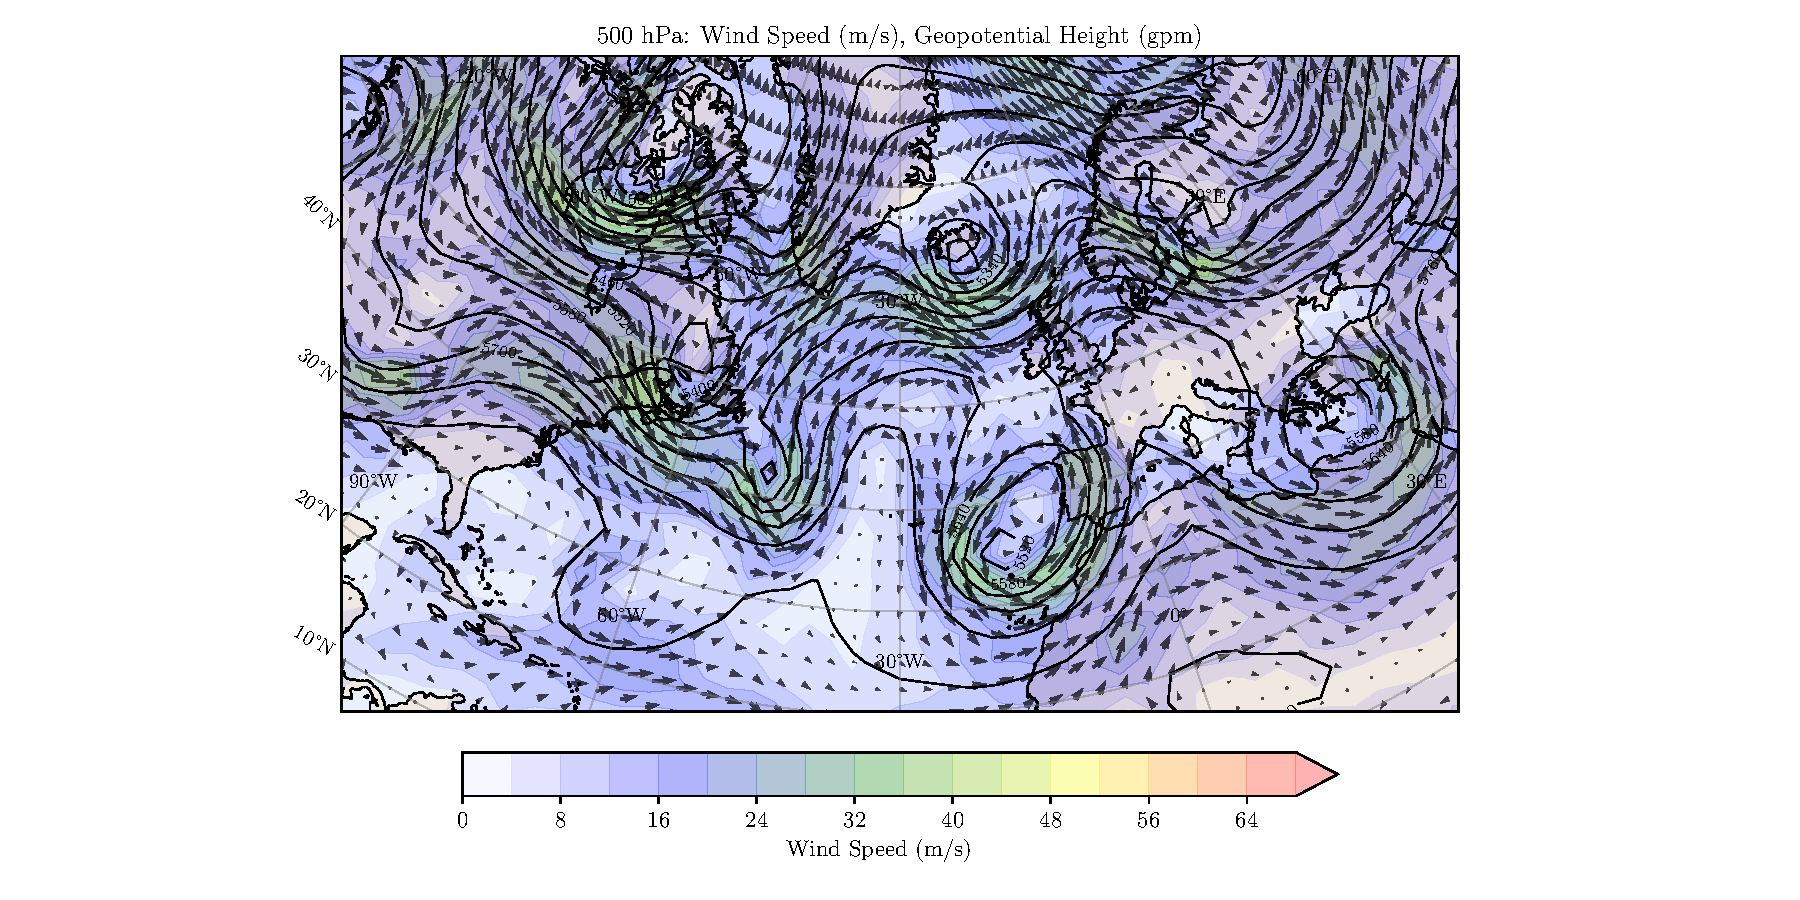
\includegraphics[width=\textwidth]{../images/weather/data_2025_5_1_00:00_500.pdf}
% \end{frame}
% \begin{frame}
%   \frametitle{Forecast: 01-May-2025 at 00:00, Level 200 hPa}
%   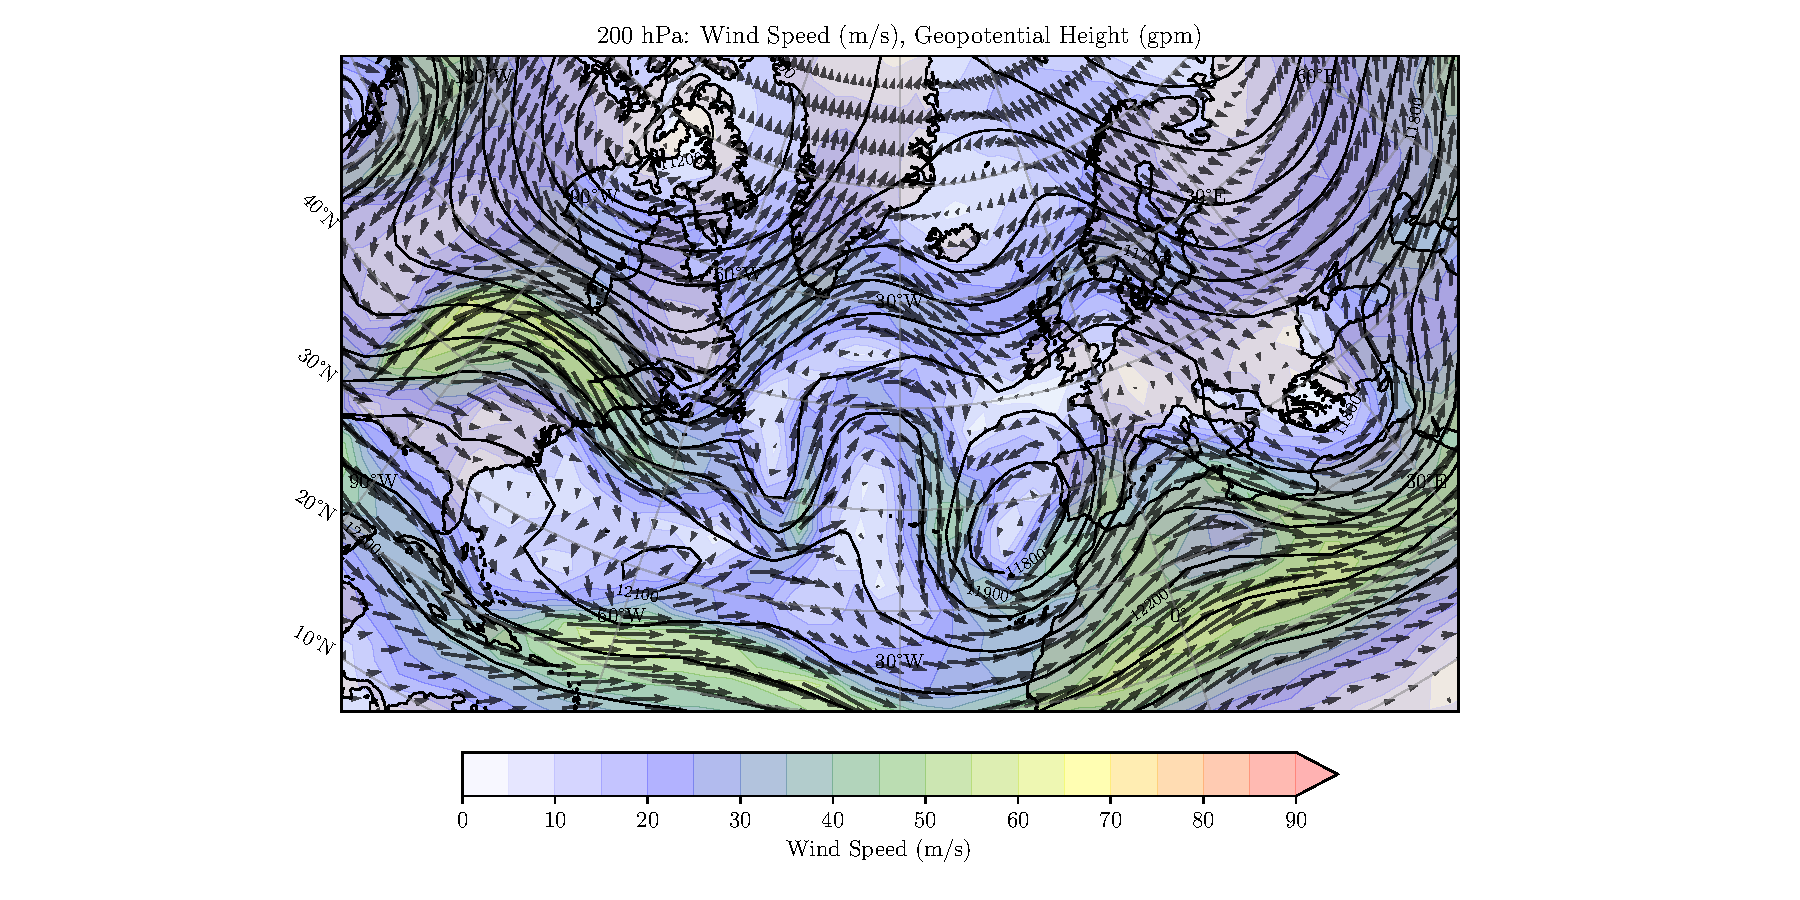
\includegraphics[width=\textwidth]{../images/weather/data_2025_5_1_00:00_200.pdf}
% \end{frame}

% In your document body:

\foreach \level in {850,500,200} {
\foreach \day in {1,...,10} {
  \foreach \time in {00:00,12:00} {
      \begin{frame}
        \frametitle{Forecast: \day-May-2025 at \time, Level \level hPa}
        \includegraphics[width=\textwidth]{../images/weather/data_2025_5_\day_\time_\level.pdf}
      \end{frame}
    }
  }
}

% In your document body:
\foreach \level in {850,500,200} {
\foreach \day in {1,...,10} {
  \foreach \time in {00:00,12:00} {
      \begin{frame}
        \frametitle{Forecast: \day-May-2025 at \time, Level \level hPa}
        \begin{center}
          \includegraphics[width=0.5\textwidth]{../images/weather/data_2025_5_\day_\time_\level_polar.pdf}
        \end{center}
      \end{frame}
    }
  }
}

\foreach \n in {01,02,03,04,05,06,07,08,09,10,
                11,12,13,14,15,16,17,18,19,20,
                21,22,23,24,25,26,27,28,29,30,
                31} {
  \begin{frame}
    \begin{center}
      \includegraphics[width=0.5\textwidth]{../images/rotating_earth/fig_\n.pdf}
    \end{center}
  \end{frame}
}
